\documentclass[compress]{beamer}
\usetheme{sthlm}

%-=-=-=-=-=-=-=-=-=-=-=-=-=-=-=-=-=-=-=-=-=-=-=-=
%        LOADING BEAMER PACKAGES
%-=-=-=-=-=-=-=-=-=-=-=-=-=-=-=-=-=-=-=-=-=-=-=-=

\usepackage{
booktabs,
datetime,
dtk-logos,
graphicx,
multicol,
pgfplots,
ragged2e,
tabularx,
tikz,
wasysym,
multirow,
float,
caption,
subcaption
}

\pgfplotsset{compat=1.8}

\usepackage[utf8]{inputenc}
\usepackage[portuguese]{babel}
\usepackage[T1]{fontenc}
\usepackage{newpxtext,newpxmath}
\usepackage{listings}

\lstset{ %
language=[LaTeX]TeX,
basicstyle=\normalsize\ttfamily,
keywordstyle=,
numbers=left,
numberstyle=\tiny\ttfamily,
stepnumber=1,
showspaces=false,
showstringspaces=false,
showtabs=false,
breaklines=true,
frame=tb,
framerule=0.5pt,
tabsize=4,
framexleftmargin=0.5em,
framexrightmargin=0.5em,
xleftmargin=0.5em,
xrightmargin=0.5em
}



%-=-=-=-=-=-=-=-=-=-=-=-=-=-=-=-=-=-=-=-=-=-=-=-=
%        LOADING TIKZ LIBRARIES
%-=-=-=-=-=-=-=-=-=-=-=-=-=-=-=-=-=-=-=-=-=-=-=-=

\usetikzlibrary{
backgrounds,
mindmap
}

%-=-=-=-=-=-=-=-=-=-=-=-=-=-=-=-=-=-=-=-=-=-=-=-=
%        BEAMER OPTIONS
%-=-=-=-=-=-=-=-=-=-=-=-=-=-=-=-=-=-=-=-=-=-=-=-=

\setbeameroption{show notes}

%-=-=-=-=-=-=-=-=-=-=-=-=-=-=-=-=-=-=-=-=-=-=-=-=
%        BEAMER COMMANDS
%-=-=-=-=-=-=-=-=-=-=-=-=-=-=-=-=-=-=-=-=-=-=-=-=


%-=-=-=-=-=-=-=-=-=-=-=-=-=-=-=-=-=-=-=-=-=-=-=-=
%
%	PRESENTATION INFORMATION
%
%-=-=-=-=-=-=-=-=-=-=-=-=-=-=-=-=-=-=-=-=-=-=-=-=

\title{Introdução a disciplina}
\subtitle{DCE692 - Pesquisa Operacional}
%\date{\small{\jobname}}
\author{\texttt{Iago Carvalho}}
\institute{\texttt{Departamento de Ciência da Computação}}

\hypersetup{
pdfauthor = {Iago A. Carvalho},      
pdfsubject = {Pesquisa Operacional},
pdfkeywords = {},  
pdfmoddate= {D:\pdfdate},          
pdfcreator = {WriteLaTeX}
}

\begin{document}

\begin{frame}
\titlepage

\end{frame}

%% --------------------------------------------------------

\begin{frame}{Pesquisa Operacional (PO)}

Pesquisa Operacional é um termo muito amplo 

\vspace{1cm}

Ele se refere a uma grande quantidade de áreas de trabalho e pesquisa

\begin{itemize}
    \item Programação matemática
    \item Simulação de produção
    \item Otimização de sistemas
    \item Apoio a tomada de decisão
    \item Teoria de jogos
    \item ...
\end{itemize}
\end{frame}

%% --------------------------------------------------------

\begin{frame}{Origens da PO}

Segunda Guerra Mundial

\begin{figure}
    \begin{overprint}
    \onslide<1>\centering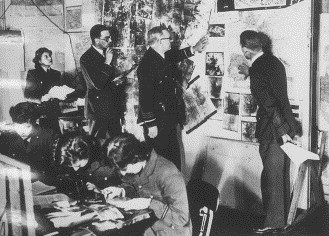
\includegraphics[width=0.80\textwidth]{images/ww2_1.jpg}
    \onslide<2>\centering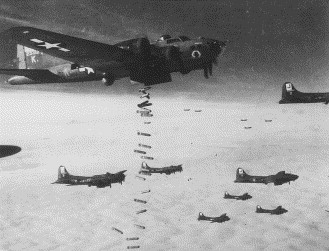
\includegraphics[width=0.80\textwidth]{images/ww2_2.jpg}
    \onslide<3>\centering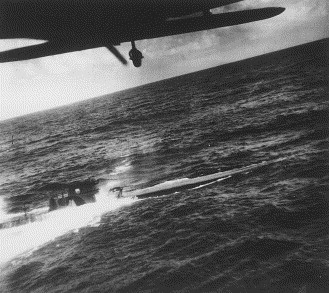
\includegraphics[width=0.80\textwidth]{images/ww2_3.jpg}
    \end{overprint}
\end{figure}
\end{frame}

%% --------------------------------------------------------

\begin{frame}{PO na Segunda Guerra}

Durante a guerra, PO foi utilizada por cientistas e matemáticos dos EUA e da Grã-Betanha para

\begin{itemize}
    \item Alocar recursos de forma eficiente
    \item Planejar movimentação de aviões e embarcações
    \item ...
\end{itemize}

\vspace{0.5cm}

Como resultado, os Aliados venceram a Batalha do Atlântico Norte e tiveram grande avanço na Campanha Britânica no Pacífico
\end{frame}

%% --------------------------------------------------------

\begin{frame}{PO no pós-guerra}
\begin{table}[]
\centering
\label{tab:my-table}
\resizebox{\textwidth}{!}{%
\begin{tabular}{@{}lll@{}}
\toprule
Organização & Aplicação & Resultados \\ \midrule
\multirow{3}{*}{Petrobrás} & \multirow{3}{*}{Planejamento de voos de helicópteros} & 18\% menos pousos e decolagens, \\
 &  & 8\% menos tempo de voo, \\
 &  & economia anual de 20 milhões de dólares \\ \midrule
\multirow{2}{*}{Samsumg} & Planejamento de linha de produção; & Economia anual de 200 milhões de dólares, \\
 & Monitoramento de estoque & dentre salários e melhora na produção \\ \midrule
\multirow{2}{*}{Peugeot e Citroen} & \multirow{2}{*}{Sequenciamento da esteira de montagem de veículos} & Economia anual de 130 milhões de dólares e \\
 &  & aumento da produção de veículos \\ \midrule
\multirow{2}{*}{Protect \& Gamble} & Redesenho do sistema de produção e & \multirow{2}{*}{Economia anual de 200 milhões de dólares} \\
 & de distribuição de itens manufaturados &  \\ \midrule
Exército dos EUA & Planejamento logístico e tático da Guerra do Golfo & Não informado \\\midrule
AT\&T & Projeto e operação de call centers & Economia anual de 750 milhões de dólares \\\midrule
Air New Zealand & Alocação de tripulação de voos & Economia anual de 6,7 milhões de dólares \\ \midrule
Taco Bell & Gerir a escala de funcionários de seus restaurantes & Economia anual de 13 milhões de dólares\\ \bottomrule
\end{tabular}%
}
\end{table}
\end{frame}

%% --------------------------------------------------------

\begin{frame}{Exemplo de uma aplicação}

FedEx - Serviço postal dos EUA 

Todos os dias, eles entregam mais de 6,5 milhões de itens
\begin{itemize}
    \item 220 países diferentes
    \item Restrições de horário 
\end{itemize}

Deve-se planejar
\begin{itemize}
    \item Rotas de aviões e navios de transporte
    \item Otimização do carregamento de aviões e navios
    \item Planejamento da rota dos entregadores
    \begin{itemize}
        \item A pé
        \item Carros
        \item Vans
        \item Motos
    \end{itemize}
    \item Alocação dos itens a serem entreges por cada entregador
\end{itemize}
\end{frame}

%% --------------------------------------------------------

\begin{frame}{Exemplo de uma aplicação}

\centering 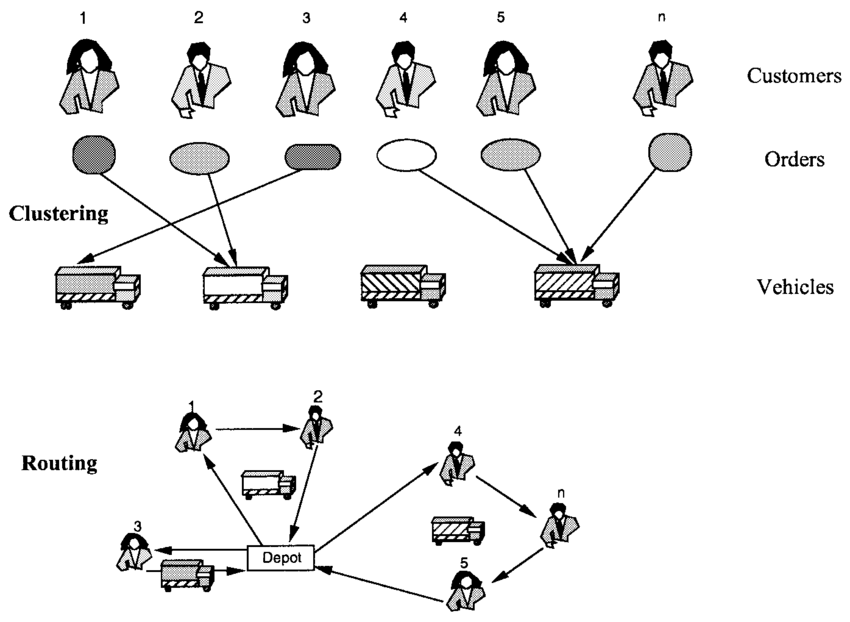
\includegraphics[width=0.95\textwidth]{images/roteamento.png}
\end{frame}

%% --------------------------------------------------------

\begin{frame}{Ferramentas de PO}

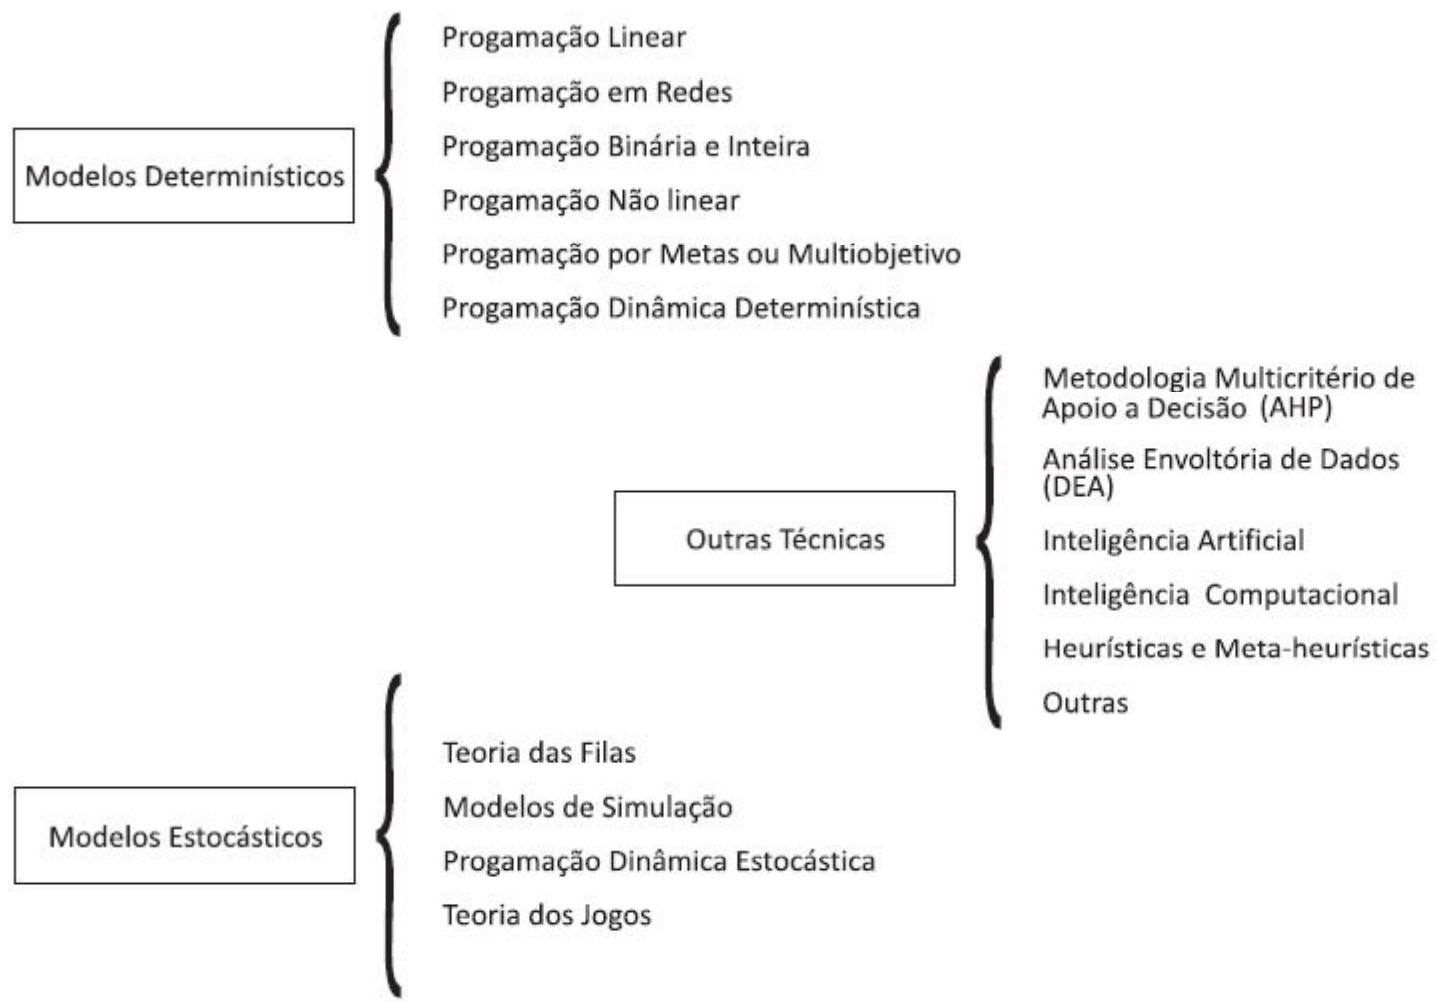
\includegraphics[width=0.95\textwidth]{images/ferramentas_po.png}

\end{frame}

%% --------------------------------------------------------

\begin{frame}{Sobre a disciplina}

Página da disciplina no Github \href{https://github.com/iagoac/dce692}{\beamergotobutton{Link}}
\end{frame}

\end{document}